\chapter[Capire la Richiesta del Cliente: Leggere da Analista]{Capire la Richiesta del Cliente:\\ Leggere da Analista}
\label{chap:comprensione-richieste}

\begin{quote}
\itshape
\small
``Molti bug non nascono da codice scritto male, ma da richieste capite male. Si risolvono con una domanda in più, non con cento righe in più.''
\end{quote}
\vspace{1em}

\noindent\textbf{Riferimento Didattico:} Lezione del 12 Ottobre 2026 -- Laboratorio di Programmazione 2\\
\textbf{Progetto Guida Annuale:} \textbf{\color{PiazzaPrimary}Vending Machine Manager} (Distributore Automatico Modulare)\\
\textbf{Competenze Chiave:} Analisi dei requisiti a partire da una richiesta in linguaggio naturale, separazione tra dati, richiesta, regole e rumore, gestione delle unità di misura, compilazione della scheda I-P-O, verifica del caso limite e formulazione delle domande per il cliente.

\vspace{1.5em}

\noindent In questo capitolo non scriviamo né codice né pseudocodice: lavoriamo sul passo che viene prima di qualsiasi classe o funzione, cioè \textbf{capire cosa vuole davvero il cliente}.

% ==============================================================================
\section{Analisi dei Requisiti: il Primo Mestiere del Programmatore}
% ==============================================================================

Le richieste per il nostro distributore arriveranno sempre così: in italiano, da una persona che non è un programmatore. Per tutto il capitolo il cliente è \textbf{Marta}, responsabile (fittizia) dei distributori della scuola.

\begin{center}
\renewcommand{\arraystretch}{1.5}
\begin{tabular}{|p{4cm}|c|p{4cm}|c|p{4cm}|}
\cline{1-1}\cline{3-3}\cline{5-5}
\cellcolor{PiazzaPrimary!10}\textbf{Il Cliente} & & \cellcolor{BoxBlue!10}\textbf{L'Analista (tu)} & & \cellcolor{BoxGreen!10}\textbf{Requisiti Chiari} \\
\small Parla come parla: mescola richieste e chiacchiere, dà per scontate molte cose, dimentica i casi strani.
 & \multicolumn{1}{c}{$\longrightarrow$} &
\small Legge, smonta e chiede: separa i dati dal rumore, traduce le regole in confronti, scrive le domande da fare.
 & \multicolumn{1}{c}{$\longrightarrow$} &
\small Nessuna ambiguità: dati con nome, valore e unità, regole precise, risultati attesi, casi limite verificati. \\
\cline{1-1}\cline{3-3}\cline{5-5}
\end{tabular}
\end{center}

\begin{attenzione}[Il Bug dei 120 Euro]
Il listino del cliente dice: \emph{``Patatine --- 120''}. Per il cliente era ovvio: \textbf{centesimi}.\\
Il programmatore capisce \textbf{120\,\euro}. Un cliente inserisce 2\,\euro{} e la macchina risponde: \emph{``Credito insufficiente, mancano 118\,\euro''}.

\smallskip
Il cliente dava per scontata l'unità di misura, il programmatore non ha chiesto.
\end{attenzione}

% ==============================================================================
\section{Lo Schema I-P-O come Filtro di Lettura}
% ==============================================================================

Lo schema Input--Elaborazione--Output (Capitolo~\ref{chap:grandi-concetti}) diventa un \textbf{filtro}: a ogni frase della richiesta chiediamo in quale casella va.

\begin{center}
\renewcommand{\arraystretch}{1.45}
\begin{tabular}{|l|l|p{6.6cm}|}
\hline
\rowcolor{PiazzaPrimary!15}
 & \textbf{Domanda da farsi} & \textbf{Cosa cercare nella richiesta} \\
\hline
\textbf{\color{BoxBlue}INPUT} & Cosa mi \textbf{dai}? & I dati che la macchina riceve o conosce: monete, prezzi, quantità. \\
\hline
\textbf{\color{BoxAmber}ELABORAZIONE} & Quali \textbf{regole}? & Calcoli e condizioni che collegano dati e risultato. \\
\hline
\textbf{\color{PiazzaPrimary}OUTPUT} & Cosa mi \textbf{chiedi}? & Cosa deve fare o mostrare la macchina alla fine. \\
\hline
\end{tabular}
\end{center}

\begin{concetto}[Il Rumore]
Tutto il resto è \textbf{\underline{rumore}}: saluti, piani dell'edificio, orari, sfoghi del cliente. Aiuta a capire il contesto (spesso spiega il \emph{perché} della richiesta), ma non entra nella scheda.
\end{concetto}

% ==============================================================================
\section{Il Metodo dell'Analista in 5 Passi}
% ==============================================================================

\begin{enumerate}
  \item \textbf{Leggi due volte.} La prima volta per capire cosa vuole il cliente, la seconda per cercare i dati.
  \item \textbf{Evidenzia} con i colori o con i simboli del kit (Sezione~\ref{sec:kit-seconda}).
  \item \textbf{Riformula} con una sola frase: \emph{``La macchina deve\dots''}.
  \item \textbf{Compila la scheda I-P-O} con nomi, valori e \textbf{unità di misura}.
  \item \textbf{Prova \& Domande:} prova con i numeri e con il \textbf{caso limite}, poi scrivi le domande per il cliente.
\end{enumerate}

\begin{concetto}[Regola d'Oro dell'Analista]
Se un dato manca, \textbf{\underline{non si inventa}}. Si chiede.
\end{concetto}

% ==============================================================================
\section{Il Kit dell'Evidenziatore: Colori e Simboli}
\label{sec:kit-seconda}
% ==============================================================================

Chi ha gli evidenziatori usa \textbf{colore e simbolo insieme}. Chi non li ha usa \textbf{solo il simbolo}, con una penna qualsiasi: ogni simbolo si disegna a mano in un secondo.

\begin{center}
\renewcommand{\arraystretch}{1.6}
\begin{tabular}{|l|l|l|p{3.5cm}|}
\hline
\rowcolor{PiazzaPrimary!15}
\textbf{Cosa cerco} & \textbf{Colore} & \textbf{Come appare} & \textbf{Simbolo a mano} \\
\hline
Dato (Input)       & blu    & \dato{0,60\,\euro}           & \textbf{cerchio}: cattura il dato \\
\hline
Richiesta (Output) & rosso  & \richiesta{dà il resto}      & \textbf{doppia sottolineatura}: il risultato \\
\hline
Regola             & giallo & \regola{se basta}            & \textbf{onda}: il bivio, la strada cambia \\
\hline
Rumore             & ---    & \rumore{simpaticissimo} & \textbf{barrato}: lo butto via \\
\hline
Dato nascosto      & blu    & \nascosto{1\,\euro{} = 100 cent} & \textbf{$\bigstar$ a margine} + il dato \\
\hline
Dato mancante      & ---    & \mancante{soglia}            & \textbf{? a margine} + la domanda per il cliente \\
\hline
\end{tabular}
\end{center}

Quando una regola contiene un confronto, lo scriviamo accanto: \regola{se il credito è sufficiente}\confronto{$\geq$}.

% ==============================================================================
\section{Il Dizionario: Parole che Diventano Confronti}
% ==============================================================================

\begin{center}
\renewcommand{\arraystretch}{1.4}
\begin{tabular}{|l|c|l|l|}
\hline
\rowcolor{PiazzaPrimary!15}
\textbf{Parola nella richiesta} & \textbf{Simbolo} & \textbf{Esempio} & \textbf{Soglia} \\
\hline
almeno                & $\geq$ & ``almeno 3\,\euro{} di credito''           & compresa \\
al massimo            & $\leq$ & ``al massimo 12 prodotti per spirale''   & compresa \\
più di / supera       & $>$    & ``supera gli 8 gradi''                   & esclusa \\
meno di / sotto       & $<$    & ``sotto i 2 pezzi''                      & esclusa \\
fino a                & $\leq$ & ``resto fino a 5\,\euro''                 & compresa \\
basta / è sufficiente & $\geq$ & ``credito sufficiente''                  & compresa \\
esattamente / pari a  & $=$    & ``importo esatto''                       & solo quella \\
diverso da / tranne   & $\neq$ & ``tutti tranne chi usa la chiavetta''    & esclusa \\
\hline
\end{tabular}
\end{center}

\begin{attenzione}[Il Caso Limite]
Prova sempre con il valore \textbf{\underline{esatto}} della soglia (3\,\euro, 5\,\euro, 8 gradi\dots). È lì che cliente e programma possono non essere d'accordo, ed è spesso lì che nasce una domanda per il cliente.
\end{attenzione}

% ==============================================================================
\section{Le 5 Trappole delle Richieste}
% ==============================================================================

\begin{enumerate}
  \item \textbf{Il rumore:} saluti, storie e numeri inutili (\emph{``comprato nel 2019, 300 bicchieri a settimana''}).
  \item \textbf{Il dato nascosto:} non è scritto, ma serve (\emph{``tre monete da 50 cent''} $\to$ $\bigstar$ credito 1,50\,\euro).
  \item \textbf{Le parole-trappola:} ``almeno'' e ``più di'' sul caso limite danno risultati opposti.
  \item \textbf{Il dato mancante:} il cliente ha dimenticato qualcosa di indispensabile (\emph{``quando sta per finire''} $\to$ quanti pezzi?).
  \item \textbf{L'unità di misura:} euro o centesimi? pezzi o confezioni? Si sceglie \textbf{una} unità e si converte tutto subito.
\end{enumerate}

% ==============================================================================
\section{Esempio Svolto: Il Resto Giusto}
% ==============================================================================

\begin{center}
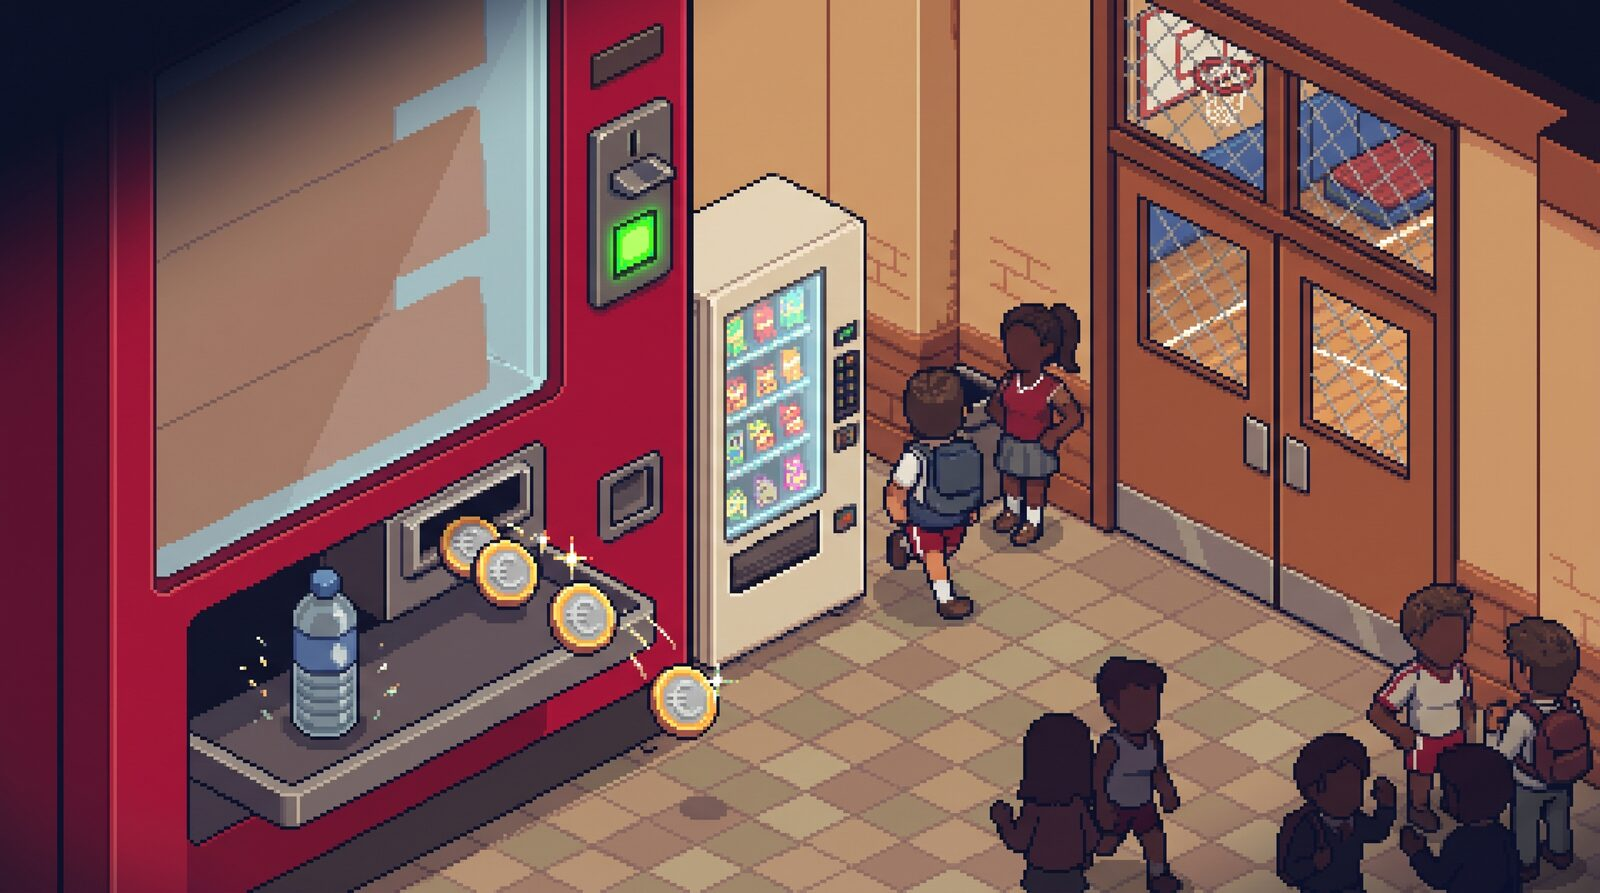
\includegraphics[width=0.8\textwidth]{../2026-10-12/presentazione/immagini/resto.jpeg}
\end{center}

\begin{esempio}[La Richiesta di Marta]
\textbf{Da:} Marta, responsabile distributori \textbullet{} \textbf{Oggetto:} distributore del piano terra

\smallskip
\emph{Ciao ragazzi! Sono Marta, gestisco i distributori del piano terra, quelli vicino alla palestra che all'intervallo delle 10:50 vengono presi d'assalto. Vorrei che la macchina, quando un cliente sceglie un prodotto, controllasse se il credito inserito è sufficiente. Se lo è, deve erogare il prodotto e restituire il resto; se non lo è, deve mostrare quanto manca. Per esempio: un cliente inserisce 2,00\,\euro{} e sceglie una bottiglietta d'acqua da 0,60\,\euro. Grazie mille e buona giornata!}
\end{esempio}

\begin{soluzione}[La Richiesta Annotata e la Scheda I-P-O]
\rumore{Ciao ragazzi! Sono Marta, gestisco i distributori del piano terra, quelli vicino alla palestra che all'intervallo delle 10:50 vengono presi d'assalto.} Vorrei che la macchina, quando un cliente sceglie un prodotto, controllasse \regola{se il credito inserito è sufficiente}\confronto{$\geq$}. Se lo è, deve \richiesta{erogare il prodotto e restituire il resto}; \regola{se non lo è}\confronto{$<$}, deve \richiesta{mostrare quanto manca}. Per esempio: un cliente inserisce \dato{2,00\,\euro} e sceglie una bottiglietta d'acqua da \dato{0,60\,\euro}. \rumore{Grazie mille e buona giornata!}

\begin{scheda}
Riformulo & \emph{``La macchina deve capire se il credito copre il prezzo e calcolare resto o importo mancante.''} \\ \hline
Input & credito = \textbf{2,00\,\euro} \textbullet{} prezzo = \textbf{0,60\,\euro} \\ \hline
Elaborazione & credito $\geq$ prezzo $\to$ resto = credito $-$ prezzo \newline altrimenti $\to$ mancano = prezzo $-$ credito \\ \hline
Output & prodotto + resto \textbf{oppure} ``Mancano X\,\euro'' \\ \hline
Prova a mano & $2{,}00 \geq 0{,}60$ \textbf{VERO} $\to$ resto $2{,}00 - 0{,}60$ = \textbf{1,40\,\euro} \newline Caso limite: credito 0,60\,\euro{} $\to$ eroga, resto 0,00\,\euro \\ \hline
Domande & ? E se il prodotto è \textbf{esaurito}? La richiesta non lo dice. \\ \hline
\end{scheda}
\end{soluzione}

% ==============================================================================
\newpage
\section{Le 5 Richieste di Marta}
% ==============================================================================

Modalità: \textbf{a coppie}. Su ogni richiesta evidenzia con colori o simboli. Sul quaderno scrivi la frase \emph{``La macchina deve\dots''}, la scheda I-P-O, la prova a mano e \textbf{almeno una domanda per Marta}.

\begin{esercizio}[Richiesta 1: Bicchierini Esauriti]
Ciao, sono ancora Marta. Il distributore delle bevande calde del primo piano è un modello vecchiotto, grigio, comprato nel 2019, e il caffè lungo è il preferito della prof di italiano. Ogni bicchierino costa alla scuola 5 centesimi e d'inverno ne usiamo circa 300 a settimana. Il problema è che, quando i bicchierini finiscono, la macchina versa lo stesso il caffè\dots{} direttamente nello scarico! Vorrei che, quando un cliente sceglie una bevanda, la macchina controllasse se c'è ancora almeno un bicchierino: se c'è, prepara la bevanda e i bicchierini diminuiscono di uno; se non c'è, non prepara niente e mostra ``Bicchieri esauriti''. Adesso nel tubo ci sono 40 bicchierini.
\end{esercizio}

\begin{esercizio}[Richiesta 2: La Gettoniera in Centesimi]
Ciao! Il tecnico della ditta, simpaticissimo, mi ha spiegato che la gettoniera nuova ragiona tutto in centesimi, mentre sul listino i prezzi sono scritti in euro. Le patatine costano 1,20\,\euro. Un cliente inserisce tre monete da 50 centesimi. La macchina deve restituire il resto usando soltanto monete da 10 centesimi. Il tecnico ha detto che ripasserà giovedì per controllare. Quante monete da 10 centesimi deve restituire la macchina?
\end{esercizio}

\begin{esercizio}[Richiesta 3: La Promo d'Autunno]
Buongiorno! Per festeggiare l'arrivo dell'autunno (e delle castagne!) lanciamo una promozione. Chi inserisce almeno 3\,\euro{} di credito riceve uno snack in omaggio; chi inserisce più di 5\,\euro{} riceve anche una bottiglietta d'acqua gratis. Attenzione: la promozione vale per tutti tranne chi paga con la chiavetta ricaricabile. Che omaggi spettano a un cliente che inserisce esattamente 5\,\euro{} in monete?
\end{esercizio}

\begin{esercizio}[Richiesta 4: L'Avviso di Rifornimento]
Ciao ragazzi, ultima richiesta della settimana, promesso! Ogni spirale della macchina snack contiene al massimo 12 prodotti. Vorrei che la macchina mi mandasse un avviso quando una spirale sta per finire, così il tecnico passa a riempirla prima che i ragazzi restino a bocca asciutta. Il tecnico di solito passa il martedì mattina. Ah, l'avviso deve arrivare anche quando una spirale è proprio vuota. Grazie!
\end{esercizio}

\begin{esercizio}[Richiesta 5: La Macchina del Secondo Piano]
Ciao a tutti! Dopo la riunione di ieri con il preside (due ore, che fatica!) abbiamo deciso: dalla prossima settimana la macchina snack del secondo piano accetterà solo monete da 50 centesimi, 1\,\euro{} e 2\,\euro. Il cliente inserisce le monete e digita il codice dello snack. Se lo snack è esaurito, la macchina restituisce tutte le monete inserite. Se invece è disponibile e il credito basta, eroga lo snack e dà il resto. Se il credito non basta, aspetta altre monete. Esempio: un cliente inserisce una moneta da 1\,\euro{} e una da 50 centesimi e digita B2, i cracker, che costano 1,30\,\euro. Nella spirale B2 ne restano 4.
\end{esercizio}

\begin{consiglio}[La Scheda I-P-O da Copiare sul Quaderno]
\begin{scheda}
Riformulo & La macchina deve \dotfill \\ \hline
Input & (nome = valore + unità) \\ \hline
Elaborazione & (calcoli e confronti) \\ \hline
Output & \\ \hline
Prova a mano & (+ caso limite) \\ \hline
Domande & (per il cliente) \\ \hline
\end{scheda}
\end{consiglio}

% ==============================================================================
\newpage
\section{Soluzioni Commentate}
% ==============================================================================

\begin{soluzione}[Richiesta 1: Bicchierini Esauriti --- trappola: il rumore]
\rumore{Ciao, sono ancora Marta. Il distributore delle bevande calde del primo piano è un modello vecchiotto, grigio, comprato nel 2019, e il caffè lungo è il preferito della prof di italiano. Ogni bicchierino costa alla scuola 5 centesimi e d'inverno ne usiamo circa 300 a settimana. Il problema è che, quando i bicchierini finiscono, la macchina versa lo stesso il caffè\dots{} direttamente nello scarico!} Vorrei che, quando un cliente sceglie una bevanda, la macchina controllasse \regola{se c'è ancora almeno un bicchierino}\confronto{$\geq$ 1}: se c'è, \richiesta{prepara la bevanda e i bicchierini diminuiscono di uno}; \regola{se non c'è}\confronto{= 0}, \richiesta{non prepara niente e mostra ``Bicchieri esauriti''}. Adesso nel tubo ci sono \dato{40 bicchierini}.

\begin{scheda}
Riformulo & \emph{``Prima di preparare, la macchina deve controllare che ci sia almeno un bicchierino.''} \\ \hline
Input & bicchierini nel tubo = \textbf{40} \textbullet{} bevanda scelta \\ \hline
Elaborazione & ``almeno uno'' $\to$ bicchierini $\geq$ 1 \newline se sì: i bicchierini scendono di 1 \\ \hline
Output & bevanda + bicchierini aggiornati \textbf{oppure} ``Bicchieri esauriti'' \\ \hline
Prova a mano & $40 \geq 1$ \textbf{VERO} $\to$ bevanda, ne restano 39. \newline Caso limite: 1 bicchierino $\to$ prepara, ne restano 0. \\ \hline
Domande & ? Se i bicchieri sono esauriti, le \textbf{monete inserite} vengono restituite? \\ \hline
\end{scheda}
Lo sfogo sul caffè nello scarico spiega il \emph{perché} della richiesta, ma non entra nella scheda. Anche i 5 centesimi e i 300 bicchieri sono numeri esca.
\end{soluzione}

\begin{soluzione}[Richiesta 2: La Gettoniera in Centesimi --- trappole: dato nascosto e unità]
Ciao! \rumore{Il tecnico della ditta, simpaticissimo, mi ha spiegato che} la gettoniera nuova \regola{ragiona tutto in centesimi}\nascosto{1\,\euro{} = 100 cent}, mentre sul listino i prezzi sono scritti in euro. Le patatine costano \dato{1,20\,\euro}. Un cliente inserisce \dato{tre monete da 50 cent}\calcolo{credito = 3 $\times$ 50}. La macchina deve restituire il resto \regola{usando soltanto monete da} \dato{10 centesimi}. \rumore{Il tecnico ha detto che ripasserà giovedì per controllare.} \richiesta{Quante monete da 10 centesimi deve restituire la macchina?}

\begin{scheda}
Riformulo & \emph{``La macchina deve calcolare il resto in centesimi e contare le monete da 10.''} \\ \hline
Input & prezzo = \textbf{1,20\,\euro} \textbullet{} monete = \textbf{3 da 50 cent} \newline taglio del resto = \textbf{10 cent} \textbullet{} $\bigstar$ 1\,\euro{} = \textbf{100 cent} \\ \hline
Elaborazione & tutto in centesimi: prezzo = 120, credito = $3 \times 50 = 150$ \newline resto = credito $-$ prezzo \textbullet{} monete = resto $\div$ 10 \\ \hline
Output & numero di monete da 10 centesimi \\ \hline
Prova a mano & $150 - 120 = 30$ cent $\to$ $30 \div 10$ = \textbf{3 monete}. \newline Errore tipico: $1{,}50 - 120$ = numero negativo! \\ \hline
Domande & ? E se il resto non è un multiplo di 10 (prezzo 1,25\,\euro)? \\ \hline
\end{scheda}
\end{soluzione}

\begin{soluzione}[Richiesta 3: La Promo d'Autunno --- trappola: le parole-trappola]
\rumore{Buongiorno! Per festeggiare l'arrivo dell'autunno (e delle castagne!)} lanciamo una promozione. Chi inserisce \regola{almeno}\confronto{$\geq$} \dato{3\,\euro} di credito riceve \richiesta{uno snack in omaggio}; chi inserisce \regola{più di}\confronto{$>$} \dato{5\,\euro} riceve anche \richiesta{una bottiglietta d'acqua gratis}. Attenzione: la promozione vale per tutti \regola{tranne chi paga con la chiavetta ricaricabile}\confronto{$\neq$}. \richiesta{Che omaggi spettano} a un cliente che inserisce \dato{esattamente 5\,\euro} \dato{in monete}?

\begin{scheda}
Riformulo & \emph{``La macchina deve decidere gli omaggi in base al credito e a come si paga.''} \\ \hline
Input & credito = \textbf{5,00\,\euro} \textbullet{} pagamento = \textbf{monete} \newline soglie: \textbf{3\,\euro} (snack) e \textbf{5\,\euro} (acqua) \\ \hline
Elaborazione & prima: pagamento $\neq$ chiavetta \newline snack se credito $\geq$ 3 \textbullet{} acqua se credito $>$ 5 \\ \hline
Output & nessun omaggio / solo snack / snack + acqua \\ \hline
Prova a mano & $5 \geq 3$ \textbf{VERO} $\to$ snack \textbullet{} $5 > 5$ \textbf{FALSO} $\to$ niente acqua. \newline Risposta: \textbf{solo lo snack}. Con la chiavetta: nessun omaggio. \\ \hline
Domande & ? Vale una volta sola per cliente? Fino a quando dura la promo? Marta voleva davvero escludere i 5\,\euro{} esatti dall'acqua? \\ \hline
\end{scheda}
\end{soluzione}

\begin{soluzione}[Richiesta 4: L'Avviso di Rifornimento --- trappola: i dati mancanti]
\rumore{Ciao ragazzi, ultima richiesta della settimana, promesso!} Ogni spirale della macchina snack contiene \regola{al massimo}\confronto{$\leq$} \dato{12 prodotti}. Vorrei che la macchina mi mandasse \richiesta{un avviso}\mancante{come e a chi?} \regola{quando una spirale sta per finire}\mancante{quanti pezzi?}, \rumore{così il tecnico passa a riempirla prima che i ragazzi restino a bocca asciutta. Il tecnico di solito passa il martedì mattina.} Ah, l'avviso deve arrivare \regola{anche quando una spirale è proprio vuota}\confronto{= 0}. \rumore{Grazie!}

\begin{scheda}
Riformulo & \emph{``La macchina deve avvisare quando i prodotti di una spirale scendono a una certa soglia.''} \\ \hline
Input & prodotti in ogni spirale \textbullet{} capienza = \textbf{12} \newline soglia = \textbf{? MANCA} \\ \hline
Elaborazione & per ogni spirale: prodotti $\leq$ soglia $\to$ avviso \newline (la spirale vuota, 0, è già compresa) \\ \hline
Output & avviso al gestore con la spirale da riempire \\ \hline
Prova a mano & Impossibile senza soglia! Se fosse 3: spirale con 3 $\to$ $3 \leq 3$ $\to$ avviso. \\ \hline
Domande & ? Quanti pezzi significa ``sta per finire''? \newline ? Avviso via email, SMS o display? Un avviso per spirale o uno riassuntivo? \\ \hline
\end{scheda}
La capienza di 12 non serve all'avviso, ma servirà al tecnico: non è rumore, è un dato per un'altra funzione.
\end{soluzione}

\begin{soluzione}[Richiesta 5: La Macchina del Secondo Piano --- tutte le trappole]
\rumore{Ciao a tutti! Dopo la riunione di ieri con il preside (due ore, che fatica!) abbiamo deciso: dalla prossima settimana} la macchina snack \rumore{del secondo piano} \regola{accetterà solo monete da 50 centesimi, 1\,\euro{} e 2\,\euro}. Il cliente inserisce le monete e digita il codice dello snack. \regola{Se lo snack è esaurito}\confronto{= 0}, la macchina \richiesta{restituisce tutte le monete inserite}. \regola{Se invece è disponibile e il credito basta}\confronto{$\geq$}, \richiesta{eroga lo snack e dà il resto}. \regola{Se il credito non basta}\confronto{$<$}, \richiesta{aspetta altre monete}\mancante{quanto?}. Esempio: un cliente inserisce \dato{una moneta da 1\,\euro} \dato{e una da 50 centesimi}\nascosto{credito 1,50\,\euro} e digita \dato{B2}, \rumore{i cracker,} che costano \dato{1,30\,\euro}. Nella spirale B2 ne restano \dato{4}.

\begin{scheda}
Riformulo & \emph{``La macchina deve scegliere tra 3 strade: rimborso, snack con resto, attesa.''} \\ \hline
Input & $\bigstar$ credito = 1 + 0,50 = \textbf{1,50\,\euro} \textbullet{} codice = \textbf{B2} \newline prezzo B2 = \textbf{1,30\,\euro} \textbullet{} quantità B2 = \textbf{4} \\ \hline
Elaborazione & 1. quantità = 0 $\to$ rimborso \newline 2. credito $\geq$ prezzo $\to$ snack + resto (credito $-$ prezzo) \newline 3. altrimenti $\to$ attesa \\ \hline
Output & rimborso / snack + resto / attesa di altre monete \\ \hline
Prova a mano & $4 \neq 0$ $\to$ disponibile \textbullet{} $1{,}50 \geq 1{,}30$ \textbf{VERO} $\to$ snack + resto \textbf{0,20\,\euro} \\ \hline
Domande & ? Per quanto tempo aspetta? \textbullet{} ? Una moneta da 20 cent viene rifiutata o tenuta? \newline ? E se in cassa non ci sono monete per il resto? \\ \hline
\end{scheda}
L'ordine delle regole conta: si controlla prima la disponibilità, poi il credito.
\end{soluzione}

% ==============================================================================
\section{Errori Tipici e Checklist dell'Analista}
% ==============================================================================

\begin{attenzione}[Gli Errori Più Comuni]
\begin{itemize}
  \item Usare tutti i numeri del messaggio (anche il 2019).
  \item Mescolare euro e centesimi nello stesso calcolo.
  \item Leggere ``almeno'' come ``più di'' (e viceversa).
  \item Inventare la soglia invece di chiederla.
  \item Dimenticare i casi che il cliente non ha scritto.
\end{itemize}
\end{attenzione}

\begin{consiglio}[Il Controllo Qualità di Ogni Nuova Funzione]
\begin{itemize}
  \item[$\square$] Ho letto la richiesta \textbf{due volte}?
  \item[$\square$] Ho \textbf{barrato} il rumore, anche i numeri che non servono?
  \item[$\square$] Ogni dato ha \textbf{nome, valore e unità di misura}?
  \item[$\square$] Ho cercato i \textbf{dati nascosti} ($\bigstar$) e quelli \textbf{mancanti} (?)?
  \item[$\square$] Ho tradotto le regole in \textbf{confronti} ($\geq$, $>$, $\leq$, $<$, $=$, $\neq$)?
  \item[$\square$] Ho provato il \textbf{caso limite}?
  \item[$\square$] Ho scritto le \textbf{domande per il cliente}?
\end{itemize}
\end{consiglio}

\begin{esercizio}[Biglietto d'Uscita: La Spia del Frigo]
Il frigorifero della macchina delle bibite deve accendere la spia di manutenzione se la temperatura interna supera gli 8 gradi. Il frigorifero è stato pulito martedì dal tecnico. In questo momento il termometro segna 8 gradi. La spia si accende?
\end{esercizio}

\begin{soluzione}[Biglietto d'Uscita: La Spia del Frigo]
Il frigorifero della macchina delle bibite deve \richiesta{accendere la spia di manutenzione} \regola{se la temperatura interna supera}\confronto{$>$} gli \dato{8 gradi}. \rumore{Il frigorifero è stato pulito martedì dal tecnico.} In questo momento il termometro segna \dato{8 gradi}. \richiesta{La spia si accende?}

\begin{scheda}
Riformulo & \emph{``La macchina deve accendere la spia solo se fa più caldo di 8 gradi.''} \\ \hline
Input & temperatura = \textbf{8 gradi} \textbullet{} soglia = \textbf{8 gradi} \\ \hline
Elaborazione & ``supera'' $\to$ temperatura $>$ 8 \\ \hline
Output & spia accesa \textbf{oppure} spia spenta \\ \hline
Prova a mano & $8 > 8$ \textbf{FALSO} $\to$ la spia resta \textbf{spenta}. \\ \hline
Domande & ? Con 8 gradi esatti Marta vuole davvero la spia spenta? \\ \hline
\end{scheda}
\end{soluzione}
